\documentclass[11pt,a4paper]{article}

\usepackage[english]{babel}
\usepackage[T1]{fontenc}
\usepackage[utf8]{inputenc}
\usepackage{graphicx}
\graphicspath{{../Figs/}}
\usepackage{float}
\usepackage{subcaption}
\usepackage[font=footnotesize,labelfont={sf,bf},textfont=sf,width=\textwidth]{caption}
\usepackage[margin=2cm]{geometry}
\usepackage[plainpages=false,pdfpagelabels,hypertexnames=false]{hyperref}
\usepackage[usenames,dvipsnames]{xcolor}
\usepackage{mathtools}
\usepackage[separate-uncertainty=true]{siunitx}
\usepackage{booktabs}


\title{\bfseries\textsc{Atomic Force Microscopy}}
\author{
Michele Masini\\ \small\texttt{\href{mailto:michele.masini@uni-ulm.de}{michele.masini@uni-ulm.de}}\and
Iyán Méndez Veiga\\ \small\texttt{\href{mailto:iyan.mendez-veiga@uni-ulm.de}{iyan.mendez-veiga@uni-ulm.de}}
}
\date{\today}


\begin{document}
\maketitle

\begin{abstract}
A compact Atomic Force Microscopy (AFM) from Nanosurf company (\href{https://www.nanosurf.com/en/products/naioafm-the-leading-compact-afm}{NaioAFM}) was used to perform measurements of the surface of three samples. Two different operation modes were used: static and tapping mode. Open source software \href{http://gwyddion.net/}{Gwyddion} was used to process the raw data.\\{\color{red} Add Motivation and finings}
\end{abstract}

\vspace{1.5cm}

\section{Introduction}

Since it was first developed in 1985 by \emph{Binning} et al., the Atomic Force Microscopy (AFM) \cite{Bhushan} has become a popular surface profiler for topographic and normal force measurements on the micro- to nanoscale. Not only AFMs, but also modified devices such as Lateral Force Microscopies (LFMs) or Friction Force Microscopies (FFMs), have found applications in different fields.

In this report, we will first describe the AFM technique, the two different operation modes that we tried (static and tapping or dynamic mode) and comment the issues we faced. And secondly, we will describe the processing of raw data obtained from the device using the open source software Gwyddion, as well as a general overview of AFM image artifacts, i.e., features which appear in the images that are not present in the original probed object.

\subsection{Theory of AFM}

AFM is quite similar to Scanning Tunneling Microscope (STM). The idea is to get 3D images of sample surfaces by using a scanning technique. Main difference between AFM and STM is that AFM can also measure insulators and it is not limited to conductors because the scanning technique does not make use of tunneling currents. Instead, AFM is able to obtain the height by measuring the ultrasmall forces that arise when the tip and the sample surface get very close to each other.

The order of magnitude of these forces is less than \SI{1}{\nano\N}. A fixed relation between these forces and the distance between the tip and the sample allows to get the profile of the surface. However, this depends on the operation mode.

\begin{figure}[ht]
\centering
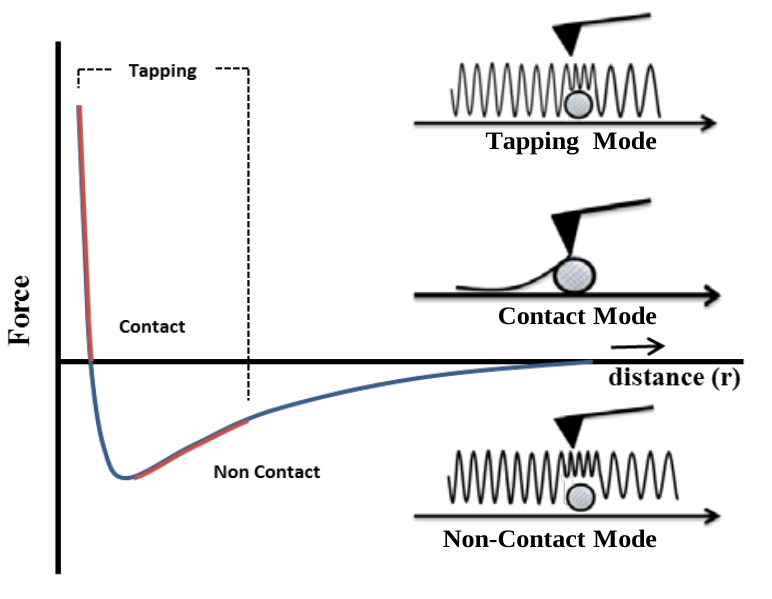
\includegraphics[width=0.7\textwidth]{AFM_modes}
\caption{Force that the tip experiments against the distance with respect to the surface of the sample \cite{jfb8010007}. In the contact mode forces are repulsive while in the non conntact mode are attractive. In the dynamic or tapping mode we are in between but typically closer to the repulsive barrier.}
\label{fig:AFM_modes}
\end{figure}

Basically, we can say that AFM can be used in two main modes or regimes (see Figure \ref{fig:AFM_modes}): static, repulsive or contact mode, and dynamic or tapping mode.

In the static mode, a sharp tip is brought into contact with the surface of the sample. The tip is placed at the end of a flexible (only in the normal direction) cantilever, which can deflect depending on the force that the tip ``feels''. The repulsive forces are due to electronic orbital overlap between the atoms of the tip and those in the surface of the sample. By measuring the deflection of the cantilever using tunneling, capacitive or optical detectors (see Figure \ref{fig:Deflection_measurement}), we can get a measure of the force if the cantilever spring constant is known.

\begin{figure}[ht]
\centering
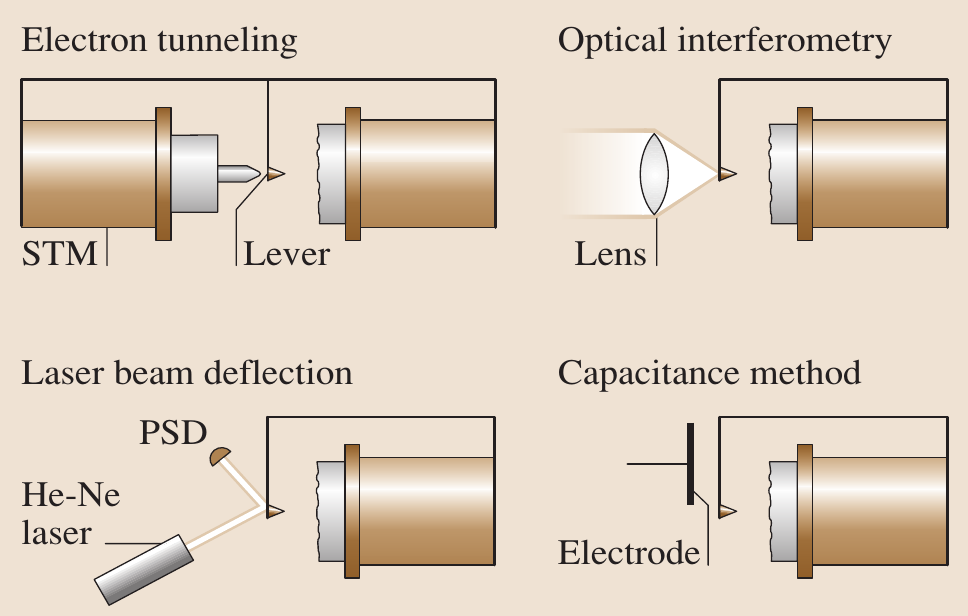
\includegraphics[width=0.5\textwidth]{Deflection}
\caption{Different techniques to measure cantilever deflection in an AFM \cite{Bhushan}.}
\label{fig:Deflection_measurement}
\end{figure}

The deflection can be measured to within \SI{0.02}{\nm}, so for a typical cantilever spring constant of \SI{10}{\N/\m}, forces as low as \SI{0.2}{\nano\N} can be measured.

Typically, the deflection of the cantilever is used as the signal for a feedback mechanism, so whenever due to the profile of the surface there is a change in this deflection, the distance $r$ between the tip and the surface of the sample is modified accordingly using a piezo material. The force that causes this aimed deflection is called \emph{setpoint} and we will see later that it is a key parameter when measuring in this mode. In order to get the profile of the whole surface, either the tip or the sample has to be translated using a piezoelectric scanner.

When we are on the right of the equilibrium (see Figure \ref{fig:AFM_modes}), the attractive forces on the tip are very weak van der Waals forces. Tapping mode can work on this regime but we do not measure the force anymore, but the force gradient. The cantilever is deliberately vibrated in either amplitude modulation (AM) or frequency modulation (FM) at its resonant frequency $\omega_0$ given by the spring constant and the force derivative is determined by measuring the shift in this resonant frequency due to the interaction with the sample.

\begin{figure}[ht]
\centering
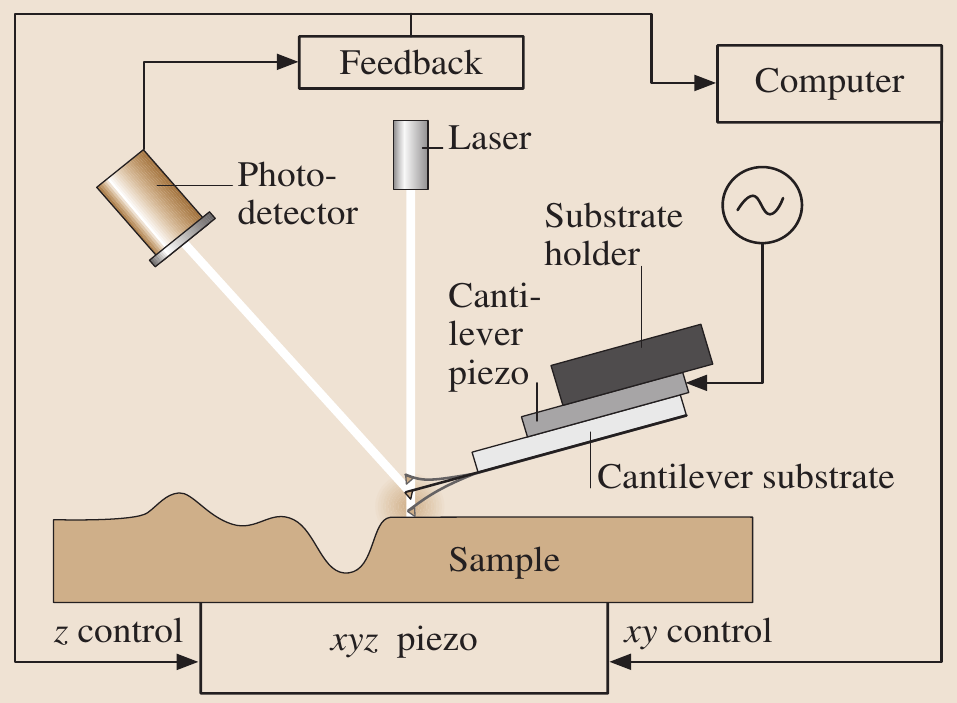
\includegraphics[width=0.5\textwidth]{Tapping_mode}
\caption{Schematic of tapping mode using a feedback mechanism to keep resonant frequency $\omega_0$ of the cantilever constant \cite{Bhushan}.}
\label{fig:Deflection_measurement}
\end{figure}

Similarly to the static mode, we can directly measure the force gradient or use this as a signal for a feedback mechanism that acts on the distance $r$ to keep constant the resonant frequency. An schematic draw is shown in Figure \ref{fig:Deflection_measurement}.

\subsection{Feedback mechanism}
We have mentioned in the previous section that the AFM can be used with or without a feedback mechanism, but since in the experiment we used it both for static and tapping modes, we will describe this technique very briefly.

Feedback mechanisms and feedback parameters are ubiquitous in our life \cite{nanosurf}. For example, when we use a thermostat, the temperature is the feedback parameter, which is set to a a desired one (\emph{setpoint}) and as the temperature in the room changes, it is compared with the temperature setpoint so that a feedback mechanism (e.g. an air conditioner) can act to keep the temperature at the desired value. Mathematically, all these mechanisms are applications of the control theory developed during the 19th century.

\begin{figure}[hbt]
\centering
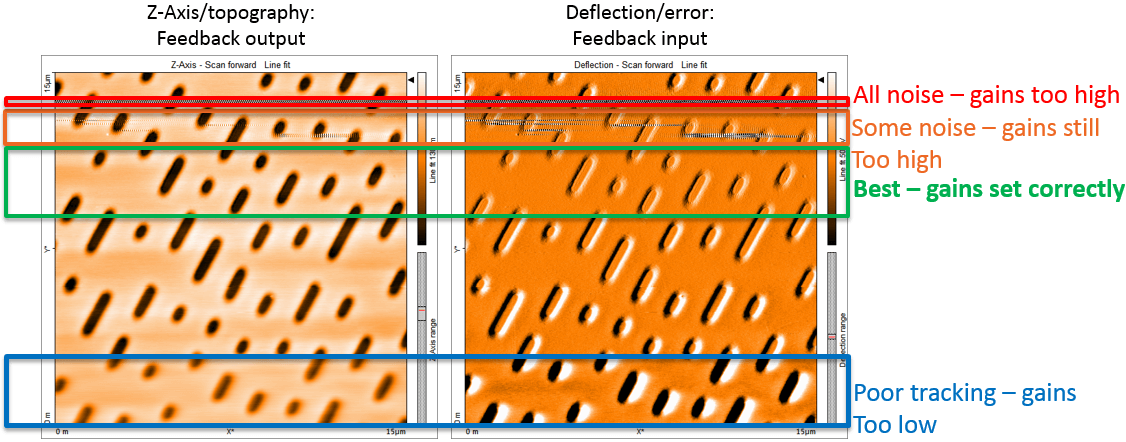
\includegraphics[width=0.8\textwidth]{afm-modes-feedback}
\caption{Feedback input and output signals for different values of PID gains \cite{nanosurf}.}
\label{fig:feedback}
\end{figure}

The feedback parameter that serves as the setpoint in contact mode is the the cantilever deflection. In the tapping mode, it is the cantilever oscillation amplitude.

The feedback mechanism is a continuous loop, the so-called feedback loop, which is controlled through the proportion-integral-derivative control, also referred as the PID gains. These different gains refer to differences in how the feedback loop adjusts to deviations from the setpoint value, i.e. the error signal. 

If gains are set too low, the PID loop is not able to keep the setpoint accurately. Contrary, if gains are chosen too high, the result will be electrical noise in the image interference from the feedback (see Figure \ref{fig:feedback}). This is due to the fact that compensation for a deviation from the setpoint is larger than the error itself.

Nevertheless, gains are not the only parameters that affect the feedback mechanism. The scan rate and, of course, the setpoint value are very important, too. If the scan rate is too fast, the PID loop will not have sufficient time to adjust the feedback parameter to its setpoint value and the height calculated from the z-piezo movement will deviate from the true topography at slopes and near edges. Very slow rates do not affect the quality of the obtained topography since they are not an issue for the PID loop, but they lead to long acquisition times.

Optimization of both scan rate and PID gains are necessary in order to optimize the feedback loop.

\subsection{AFM artifacts}
When using an AFM, as well as in many other experiments, we may find features which appear in the obtained images that are not present in the observed sample. These are called artifacts \cite{artifacts} and there are four primary sources of artifacts in images measured with AFMs: probes, scanners, image processing and vibrations.

\begin{figure}[ht]
\centering
\begin{subfigure}[b]{0.45\textwidth}
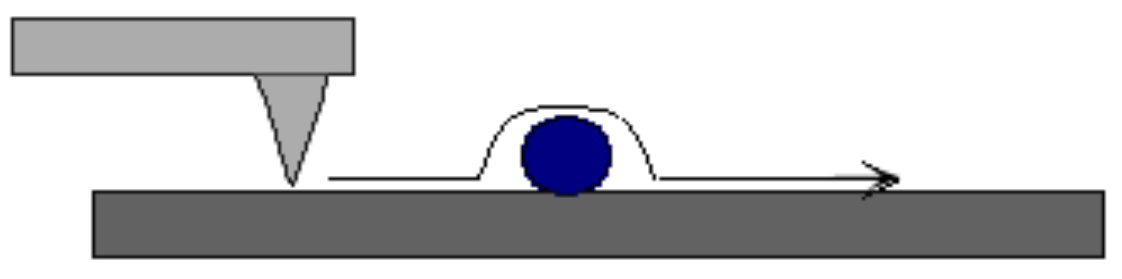
\includegraphics[width=\textwidth]{artifacts_probe_1}
\caption{Feature appears too large}
\label{fig:artifacts_probe_1}
\end{subfigure}
\begin{subfigure}[b]{0.45\textwidth}
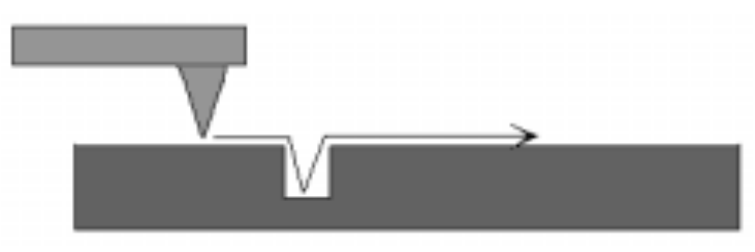
\includegraphics[width=\textwidth]{artifacts_probe_2}
\caption{Feature appears too small}
\label{fig:artifacts_probe_2}
\end{subfigure}\\\vspace{.2cm}
\begin{subfigure}[b]{0.45\textwidth}
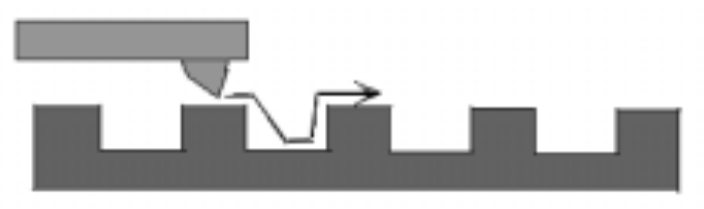
\includegraphics[width=\textwidth]{artifacts_probe_3}
\caption{Distorsion caused by a chipped tip}
\label{fig:artifacts_probe_3}
\end{subfigure}
\caption{Some examples of probe-generated artifacts \cite{artifacts}.}
\label{fig:artifacts_probe}
\end{figure}

Images measured with an AFM are always a convolution of the probe geometry and the shape of the features being imaged. In order to avoid probe-generated artifacts, the tip should be much smaller than the features being measured. When this condition is not satisfied or if the tip is damaged, features on the sample may appear larger, smaller or with strangely shaped patterns as shown in Figure \ref{fig:artifacts_probe}.

Artifacts may also arise due to the motion of the scanner in the X, Y and Z directions. Piezoelectric materials move in a nonlinear motion when a linear voltage ramp is applied. If they are not well calibrated, sizes and forms my appear severely distorted (see Figure \ref{fig:artifacts_scanner_1}). Besides, the geometry of the scanner and the positioning of it relative to the sample can also create artifacts (see Figure \ref{fig:artifacts_scanner_2}).

\begin{figure}[H]
\centering
\begin{subfigure}[b]{0.45\textwidth}
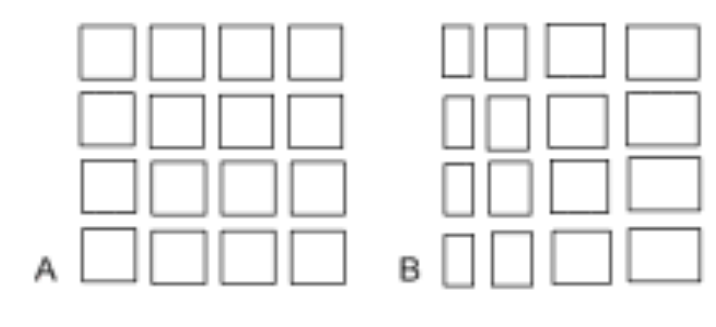
\includegraphics[width=\textwidth]{artifacts_scanner_1}
\caption{A test pattern with squares (left) distorted in the AFM (right) due to nonlinearity of the piezo materials}
\label{fig:artifacts_scanner_1}
\end{subfigure}
\begin{subfigure}[b]{0.45\textwidth}
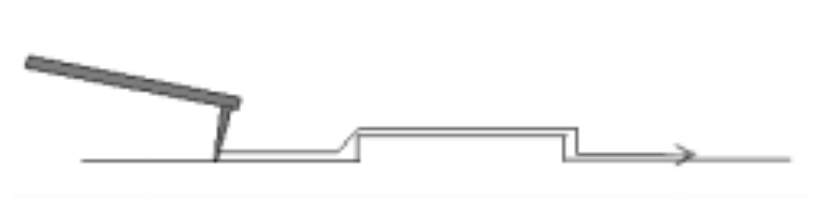
\includegraphics[width=\textwidth]{artifacts_scanner_2}
\caption{Artifact due to the probe sample angle}
\label{fig:artifacts_scanner_2}
\end{subfigure}\\\vspace{.2cm}
\begin{subfigure}[b]{0.45\textwidth}
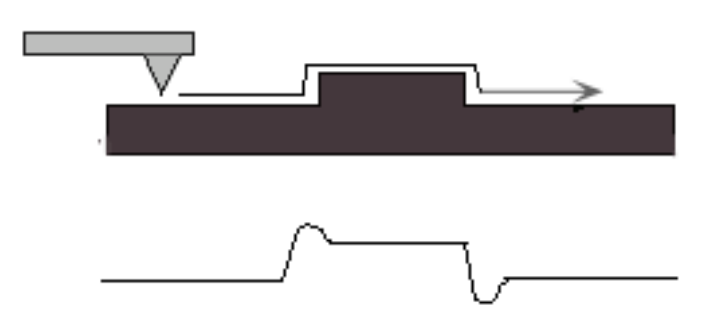
\includegraphics[width=\textwidth]{artifacts_scanner_3}
\caption{Artifact due to overshoot at the leading and trailing edge}
\label{fig:artifacts_scanner_3}
\end{subfigure}
\caption{Some examples of scanner-generated artifacts \cite{artifacts}.}
\label{fig:artifacts_scanner}
\end{figure}

Processing images is a must when dealing with AFM, but additional artifacts can be introduced if the processing software is not properly used. For example, bands that do not correspond to a real structure may appear when subtracting the background (see Figure \ref{fig:artifacts_processing}).

\begin{figure}[H]
\centering
\begin{subfigure}[b]{0.3\textwidth}
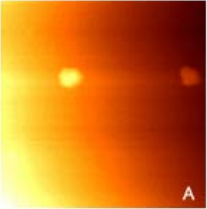
\includegraphics[width=\textwidth]{artifacts_processing_1}
\caption{Image obtained from AFM before any processing}
\label{fig:artifacts_processing_1}
\end{subfigure}
\begin{subfigure}[b]{0.3\textwidth}
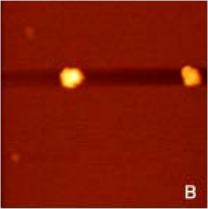
\includegraphics[width=\textwidth]{artifacts_processing_2}
\caption{After a line-by-line leveling with a background correction}
\label{fig:artifacts_processing_2}
\end{subfigure}
\begin{subfigure}[b]{0.3\textwidth}
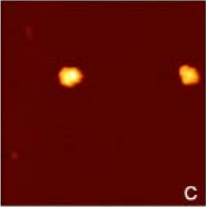
\includegraphics[width=\textwidth]{artifacts_processing_3}
\caption{Particles excluded from the background subtraction}
\label{fig:artifacts_processing_3}
\end{subfigure}\\\vspace{.2cm}
\begin{subfigure}[b]{0.6\textwidth}
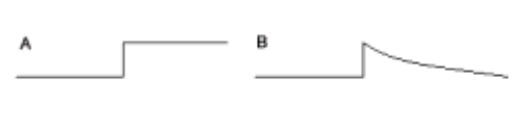
\includegraphics[width=\textwidth]{artifacts_processing_4}
\caption{Artifact due to overshoot at the leading and trailing edge}
\label{fig:artifacts_processing_4}
\end{subfigure}
\caption{Some examples of processing-generated artifacts \cite{artifacts}.}
\label{fig:artifacts_processing}
\end{figure}

Vibrations caused by sound waves can also cause artifacts. Even though the NaioAFM has an isolated compartment to avoid that, even noise derived from a person talking in the same room as the AFM can be observed (see Figure \ref{fig:artifacts_vibrations}). Additionally, surface contamination on the sample (see Figure \ref{fig:artifacts_contamination})or electronic noise (see Figure \ref{fig:artifacts_electronics}) among others can also cause artefacts.

\begin{figure}[H]
\centering
\begin{subfigure}[b]{0.45\textwidth}
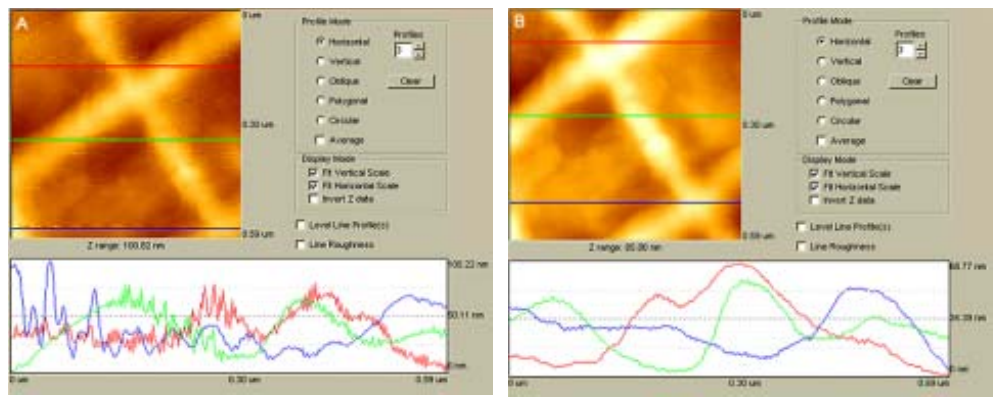
\includegraphics[width=\textwidth]{artifacts_vibrations}
\caption{Without noise (left) and with noise (right)}
\label{fig:artifacts_vibrations}
\end{subfigure}
\begin{subfigure}[b]{0.45\textwidth}
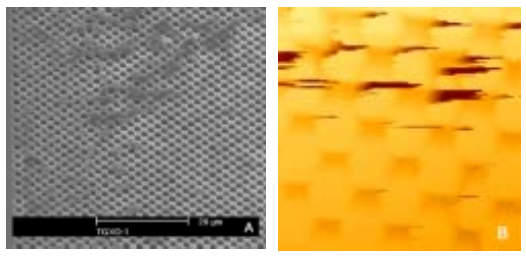
\includegraphics[width=\textwidth]{artifacts_contamination}
\caption{Sample contamination shown in a SEM image (left) and in an AFM one (right)}
\label{fig:artifacts_contamination}
\end{subfigure}\\\vspace{.2cm}
\begin{subfigure}[b]{0.45\textwidth}
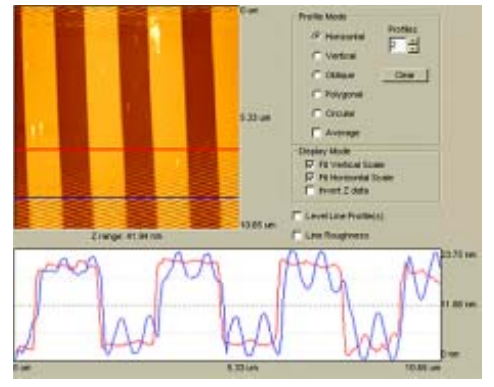
\includegraphics[width=\textwidth]{artifacts_electronics}
\caption{Electronic noise}
\label{fig:artifacts_electronics}
\end{subfigure}
\caption{Some examples of artifacts caused by sound noise, contamination and electronic noise \cite{artifacts}.}
\label{fig:artifacts_others}
\end{figure}

\section{Materials and methods}

\subsection{NaioAFM}

The NaioAFM by Nanosurf \cite{NaioAFM} is the AFM used in this experiment. As the successor of the Easyscan 2, the NaioAFM is a compact AFM designed for new and inexperienced AFM users. It has a closed scanner compartment that helps with acoustic and air current isolation, stage positioners to adjust your sample. The different parts of the scan head including the spot for the cantilever are shown in the Figure \ref{fig:naioafm}. The NaioAFM was placed on an isolation platform to avoid vibration disturbances.

\begin{figure}[hbt]
\centering
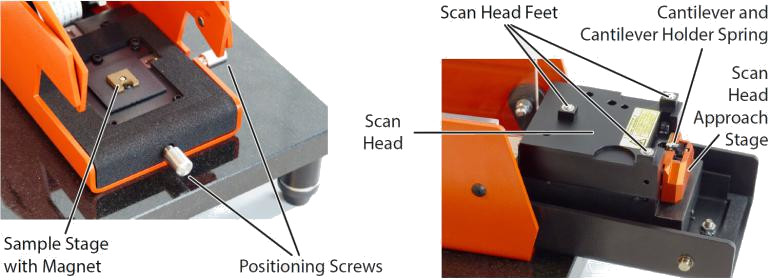
\includegraphics[width=0.9\textwidth]{naioafm2}
\caption{Different parts of the scan head of the NaioAFM instrument \cite{NaioAFM}.}
\label{fig:naioafm}
\end{figure}

A diagram of the specific feedback mechanism of the Z-controller that the NaioAFM implements can be seen in Figure \ref{fig:feedback_z-controller}.

\begin{figure}[hbt]
\centering
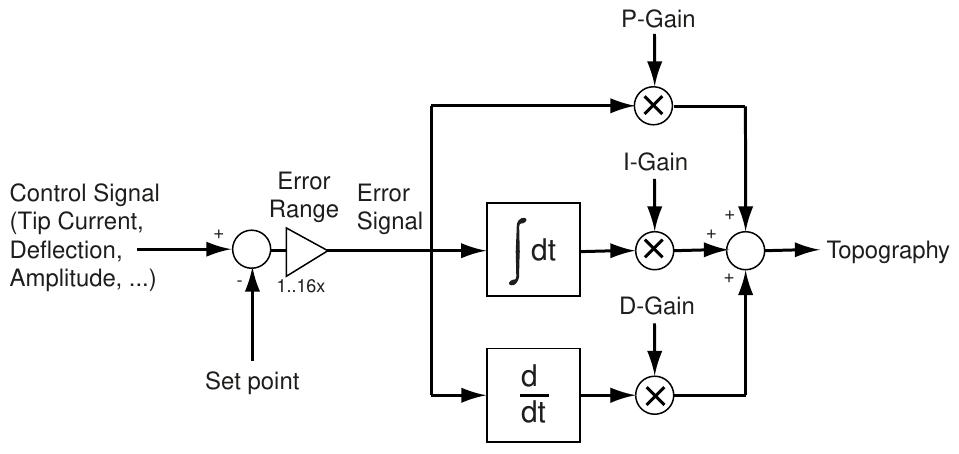
\includegraphics[width=0.8\textwidth]{Feedback_NaioAFM}
\caption{Diagram of the Z-controller of the NaioAFM from the instrument's manual.}
\label{fig:feedback_z-controller}
\end{figure}

Using this loop, the NaioAFM continuously tries to keep this feedback parameter constant at its setpoint by adjusting the z-piezo to move the cantilever probe up and down. And the resulting z-piezo movements provide the height information to create the surface topography.

According to the owner's manual from Nanosurf, the integral gain is the most important gain value and can have a dramatic effect on the image quality. The proportional gain might provide slight improvement only after the integral gain has been optimized. And the derivative gain is mainly for samples with tall edges.

Regarding the tips, we use two different types, both made of Silicon nitride (Si$_3$N$_4$): \texttt{PPP-CONTR-20} for the static mode and \texttt{Tap190Al-G} for tapping mode.

\subsection{Calibration sample}

Thes sample used to test and optimize parameters of the NaioAFM was the Calibration Standard \texttt{HS-100MG}, whcih has six different surfaces (see Figure \ref{fig:HS-100MG}).

\begin{figure}[H]
\centering
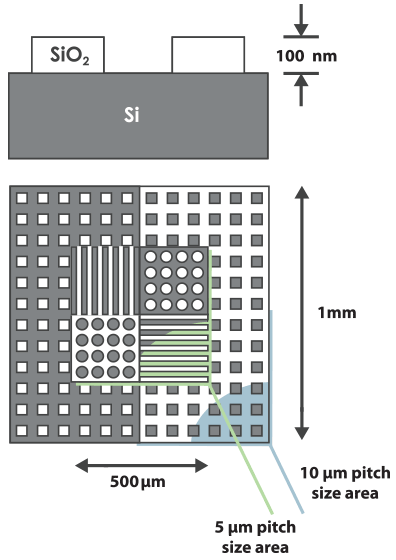
\includegraphics[width=0.4\textwidth]{HS-100MG}
\caption{Dimensions of the calibration sample HS-100MG.}
\label{fig:HS-100MG}
\end{figure}

\subsection{Gwyddion}

NaioAFM saves the data obtained by the samples in \texttt{.nid} files. These files contain 3-dimensional data of the sample: to every point in the (x,y) plane there is an associated height. The height is shown in 2-dimensional heatmaps using a gray colormap. The lighter the gray, the higher the z point is (see Figure \ref{fig:heatmap_rawdata}.)

It is possible to partially correct the noisy parts of the pictures manually or by means of some automatic tools. The data can be levelled by subtracting the mean plane; this corrects situations like the one shown in Figure~\ref{fig:artifacts_processing_1}. Secondly, it is possible to align the raws horizontally or vertically evaluating the median of the differences between them (the error that this tool is able to correct is shown in Figure~\ref{fig:artifacts_processing_2}). A third tool often used is the correction of the horizontal scars.

Moreover, the software allow us to model the colour scale by selecting the height range (Figure~\ref{fig:scale_selection}) and to set the 0 of the z-axis.

\begin{figure}[ht]
\centering
\begin{subfigure}[b]{0.45\textwidth}
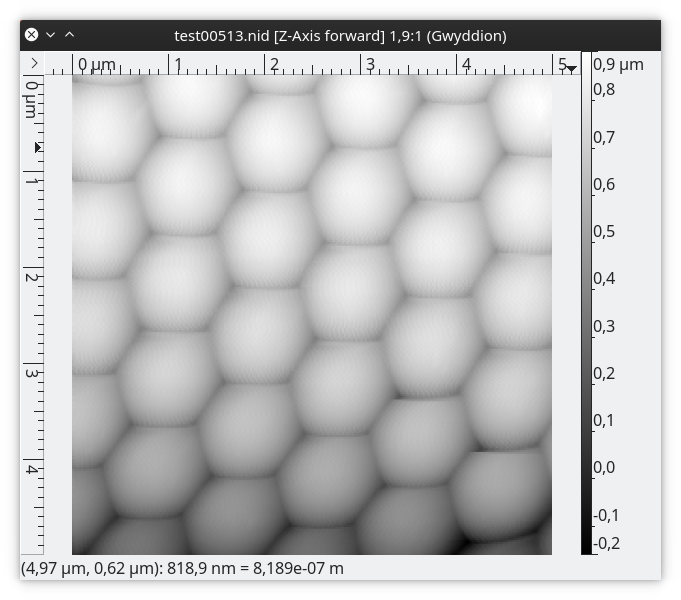
\includegraphics[width=\textwidth]{heatmap_rawdata}
\caption{Raw heatmap shown in Gwyddion after importing raw data from NaioAFM without any processing.}
\label{fig:heatmap_rawdata}
\end{subfigure}
\begin{subfigure}[b]{0.45\textwidth}
\centering
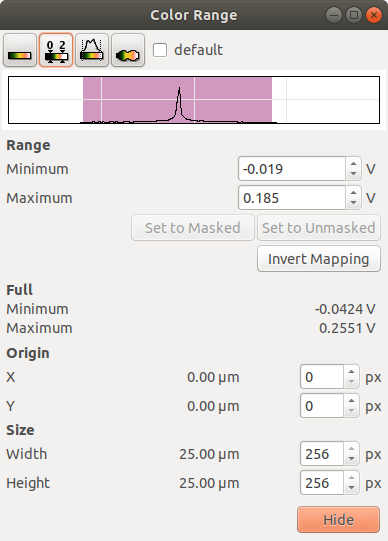
\includegraphics[width=0.7\textwidth]{scale_selection}
\caption{Selection of the highnesses interval}
\label{fig:scale_selection}
\end{subfigure}
\caption{Some screenshots of Gwyddion.}
\label{fig:gwyddion}
\end{figure}

Finally, Gwyddion allows us to improve the aesthetics of the images, making them more intuitive. First of all, we can select the colour scale which labels the height of the picture. Secondly, the software is able to generate a 3-dimensional pictures of the sample, as we will see in the following section.

\section{Results and discussion}
In this section we will describe the analysis of the three samples using static and tapping mode. 

\subsection{Static mode}
\subsubsection{Calibration}
First, we used the \emph{calibration sample} with a known surface in order to test the tip and the software used to obtain our data. 

We fixed the sample in the centre of the AFM and used the camera installed inside our Nanosurf NaioAFM equipment to place the tip in the different surfaces (shown in Figure~\ref{fig:cal_sam}).

\begin{figure}[ht]
\centering
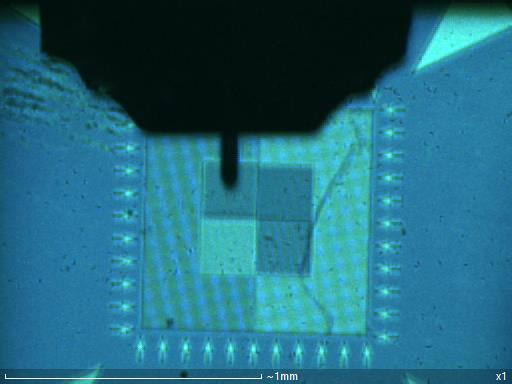
\includegraphics[scale=0.4]{calibration_sample}
\caption{Calibration sample view from the camera installed in Nanosurf NaioAFM}
\label{fig:cal_sam}
\end{figure}

Once we had chosen the surface which we wanted to analyse, by using the software, we moved the tip as close as possible to the sample, without making them contact. Then, using the \emph{approach mode}, we brought the tip in contact with the surface. This mode uses the setpoint and the feedback mechanism to very slowly put the tip in contact minimizing the risk of breaking the tip.

The key parameter we tried to optimize was the setpoint. In the software, the setpoint is express in \si{\nano N} and it is calculated by multiplying the deflection with the spring constant of the selected cantilever, which we had to choose before doing anything. A setpoint too high may damage the tip. We did eight measurements with setpoints from \SI{2}{\nano N} to \SI{20}{\nano N}. We did not have time to optimize the PID values so we used the default and suggested ones: $\text{I-Gain}=1000$ and $\text{P-Gain}=1000$.

In the Figure \ref{fig:static_calibration_grid}, three different shapes captured from our calibration sample are shown. The obtained height of the patterns was between \SI{107}{\nano m} and \SI{110}{\nano n} after some processing using the read value tool for some random positions of the pictures (see screenshot \ref{fig:read_tool}). It is possible to observe the x-scale on the top of the pictures, the y-scale on the left and the height colour scale on the right.

\begin{figure}[H]
\centering
\begin{subfigure}[b]{0.45\textwidth}
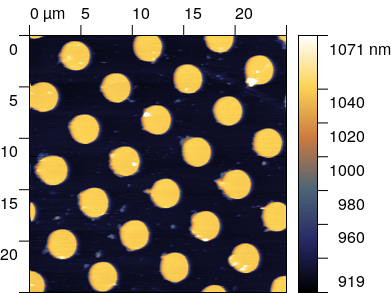
\includegraphics[width=\textwidth]{sm_points}
\caption{Points surface}
\label{fig:sm_points}
\end{subfigure}
\begin{subfigure}[b]{0.45\textwidth}
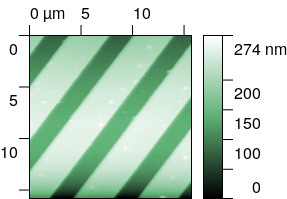
\includegraphics[width=\textwidth]{sm_raws}
\caption{Raws surface}
\label{fig:sm_raws}
\end{subfigure}\\\vspace{.2cm}
\begin{subfigure}[b]{0.45\textwidth}
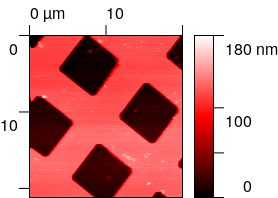
\includegraphics[width=\textwidth]{sm_squares}
\caption{Squares surface}
\label{fig:sm_squares}
\end{subfigure}
\begin{subfigure}[b]{0.45\textwidth}
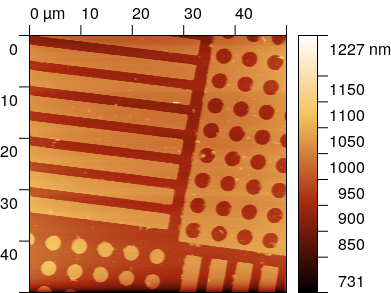
\includegraphics[width=\textwidth]{sm_border}
\caption{Border between more surfaces}
\label{fig:sm_border}
\end{subfigure}
\caption{Some pictures of the calibration sample}
\label{fig:static_calibration_grid}
\end{figure}

\begin{figure}[H]
\centering
\begin{subfigure}[b]{0.45\textwidth}
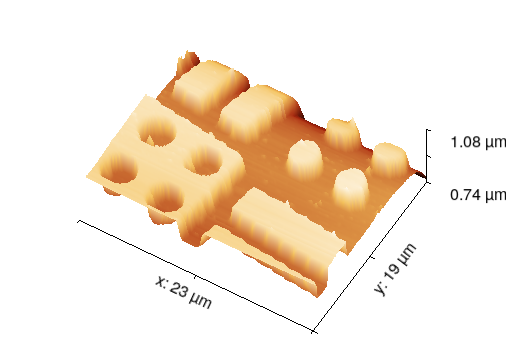
\includegraphics[scale=0.47]{sm_border_3D}
\caption{3D plot of the calibration sample's border}
\label{fig: cal sam border}
\end{subfigure}
\begin{subfigure}[b]{0.45\textwidth}
\centering
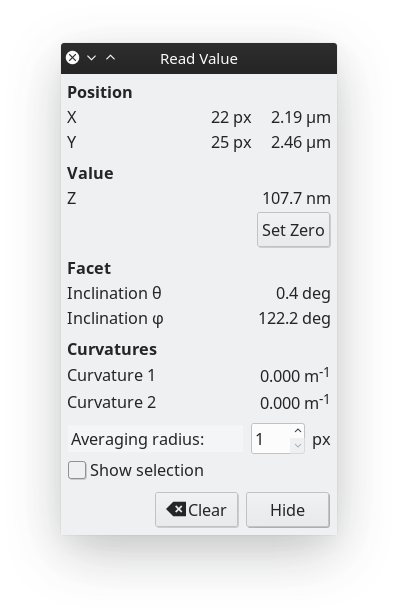
\includegraphics[width=0.6\textwidth]{static_mode_read_value_height}
\caption{Read tool to obtain height value}
\label{fig:read_tool}
\end{subfigure}
\caption{3D plot of the calibration sample's border}
\label{fig:3d_and_read_value}
\end{figure}

The previous pictures have been processed using Gwyddion software. First of all we used some masks to eliminate automatically some imperfections, as for instance orizontal tears caused by abrupt movements of the tip. Secondly, we adjusted the high scale in which the shade of colors had to variate. Finally, we chose four different colour scales in order to better distinguish the four pictures.

We can notice that the lenght scale of the pictures on the top and on the sides. Additionally, a 3D image from the data taken in the border can be seen in Figure \ref{fig: cal sam border}.

\subsubsection{Sample 1}
The first sample was labelled as \texttt{Cr \SI{2}{\nano m}, Al \SI{20}{\nano m}}. We were able to make one measurement in the dark part of the sample before having some issues doing the approach (see Figure \ref{fig:sample1_first_tip}). We decided to change the tip but the next measurement (Figure \ref{fig:sample1_second_tip}) suffered from an distorsion, an artifact probably due to a certain angle between the tip and the sample's surface as shown previoulsy in Figure \ref{fig:artifacts_scanner_2}.

\begin{figure}[H]
\centering
\begin{subfigure}[b]{0.45\textwidth}
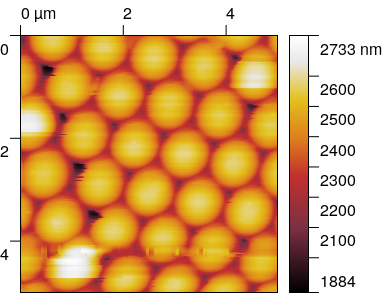
\includegraphics[width=\textwidth]{sm_sample1}
\caption{Sample 1 with first tip}
\label{fig:sample1_first_tip}
\end{subfigure}
\begin{subfigure}[b]{0.45\textwidth}
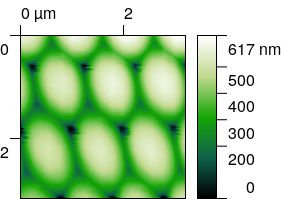
\includegraphics[width=\textwidth]{sm_sample1_dir2}
\caption{Clear artifact with the same sample 1}
\label{fig:sample1_second_tip}
\end{subfigure}\\\vspace{.2cm}
\begin{subfigure}[b]{0.45\textwidth}
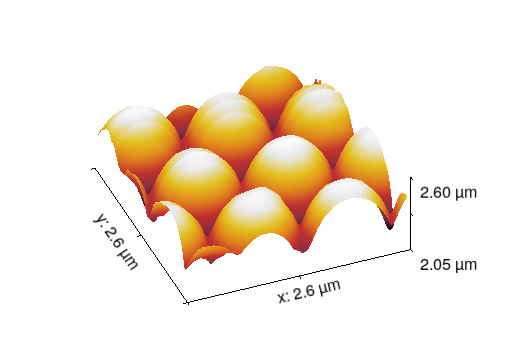
\includegraphics[width=\textwidth]{sm_sample1_3D}
\caption{3D plot of the first measurement}
\label{fig:}
\end{subfigure}
\begin{subfigure}[b]{0.45\textwidth}
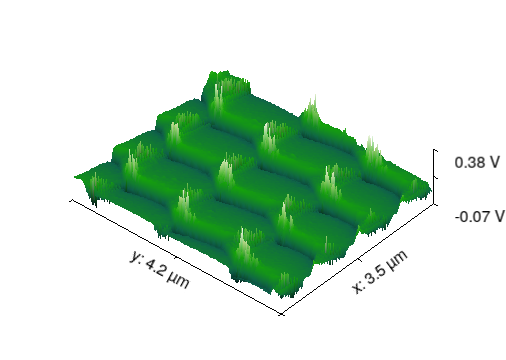
\includegraphics[width=\textwidth]{sm_sample1_dir2_3D}
\caption{3D plot of the second measurement}
\label{fig:}
\end{subfigure}
\caption{Sample 1}
\end{figure}

We can see from the two measurements that we have some kind of honeycomb structure with spheres of height $\sim\SI{0.5}{\micro m}$.

\subsubsection{Sample 2}
We did not have enough time to measure sample 2 in the static mode. Results for this sample are shown in the tapping mode section.

\subsubsection{Sample 3}
The third sample contained gold particles in silicon dioxide. We can see from Figure \ref{fig:sample_3_static} that the surface of this material was scratched and with some imperfections.

\begin{figure}[ht]
\centering
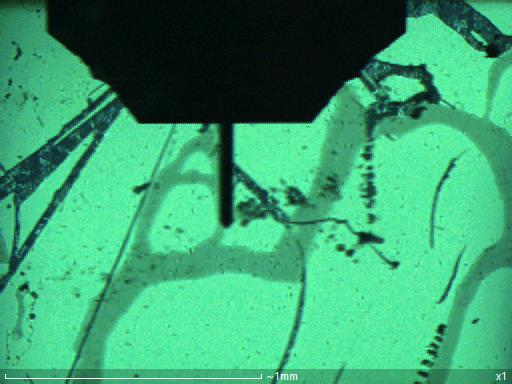
\includegraphics[scale=0.4]{sm_sample2_set.JPG}
\caption{Picture of sample 3 from the camera installed in Nanosurf NaioAFM}
\label{fig:sample_3_static}
\end{figure}

We noticed two distinguishable parts in the sample: light and dark green. We first decide to measure in the dark green areas and in the frontier between dark and green as shown in Figure \ref{fig:sample_3_static}.

\begin{figure}[H]
\centering
\begin{subfigure}[b]{0.45\textwidth}
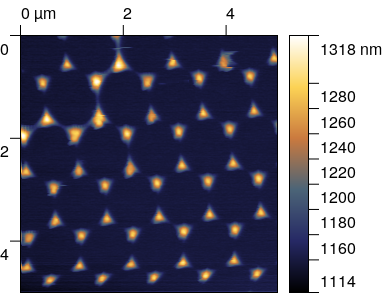
\includegraphics[width=\textwidth]{sm_sample2}
\caption{Sample 2: inside the plot}
\label{fig:sample2}
\end{subfigure}
\begin{subfigure}[b]{0.45\textwidth}
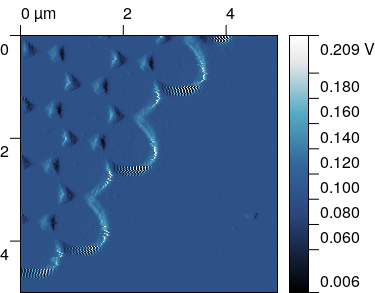
\includegraphics[width=\textwidth]{sm_sample2_border}
\caption{Sample 2: border}
\label{fig:}
\end{subfigure}\\\vspace{.2cm}
\begin{subfigure}[b]{0.45\textwidth}
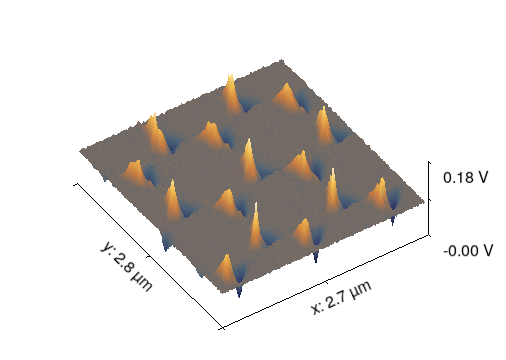
\includegraphics[width=\textwidth]{sm_sample2_3D}
\caption{Sample 2: inside the plot, 3D plot}
\label{fig:}
\end{subfigure}
\begin{subfigure}[b]{0.45\textwidth}
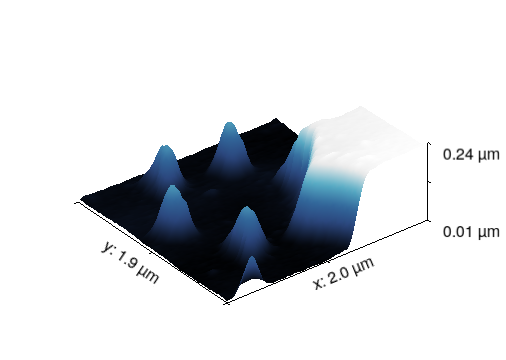
\includegraphics[width=\textwidth]{sm_sample2_border_3D}
\caption{Sample 1: border, 3D plot}
\label{fig:}
\end{subfigure}
\caption{Sample 2}
\end{figure}

We can observe that the plot reminds a set of stars. Moreover, we can see that the surface outside this plot is flat compared to the edges of the star. This triangle patterns may be an artifact due to the fact that the tip is as big as the feature in the surface we are trying to observe. We think that this corresponds to the golden particles.

Then we decide to measure only in the lighter part. We took only one measurement in the center of the light green part as shown in Figure \ref{fig:sample3_light_green_cam}. In this measurement (see Figure \ref{fig:sample3_light_green}) we can notice a hilly surface, but without the interesting pattern found in the dark areas of the sample.

\begin{figure}[ht]
\centering
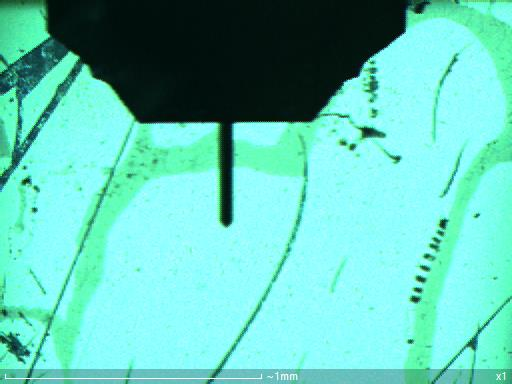
\includegraphics[scale=0.4]{sm_sample3_set}
\caption{Picture of sample 3 from the camera installed in Nanosurf NaioAFM}
\label{fig:sample3_light_green_cam}
\end{figure}

\begin{figure}[H]
\centering
\begin{subfigure}[b]{0.45\textwidth}
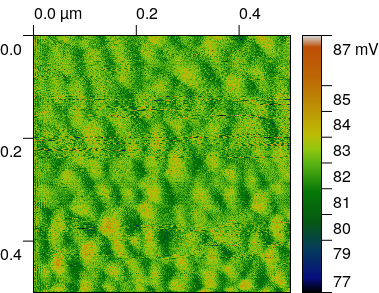
\includegraphics[width=\textwidth]{sm_sample3}
\caption{Sample 3: inside the plot}
\end{subfigure}
\begin{subfigure}[b]{0.45\textwidth}
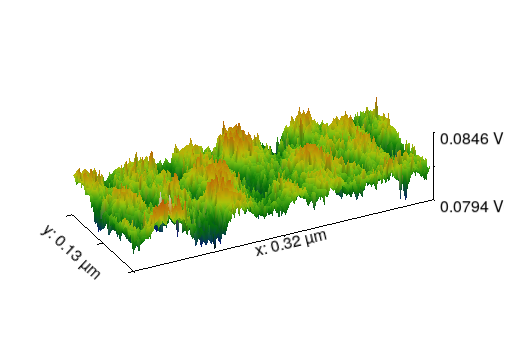
\includegraphics[width=\textwidth]{sm_sample3_3D_improved}
\caption{Sample 3: 3D plot}
\end{subfigure}
\caption{Sample 3}
\label{fig:sample3_light_green}
\end{figure}

\subsection{Tapping mode}
After changing the tip, the first thing we had to do was find the frequency of the cantilever. This was done automatically by the NaioAFM software with the \emph{Frequency Sweep} procedure.

\subsubsection{Calibration}
Once again, the first step was the measurement of the calibration sample. For the default gain values ($\text{P-Gain}=1000$ and $\text{I-Gain}=1000$), we did several measurements with different values of the setpoint. In this case, it is not a force (in \si{\nano N}) anymore like in the static mode, but a percentage that represents the threshold in the reduction of the oscillation's amplitude. For example, a setpoint of 60\% means that the Z-controller will move the tip closer to the sample until the vibration amplitude has decreased to 60\% of the vibration amplitude when it is far away from the sample.

With the calibration grid we tried setpoints of 45\%, 50\%, 65\% and 75\%. We fixed the setpoint at 45\% and then we tried to optimize the PID values. We only noticed differences by varying the I-Gain value.


\begin{figure}[H]
\centering
\begin{subfigure}[b]{0.45\textwidth}
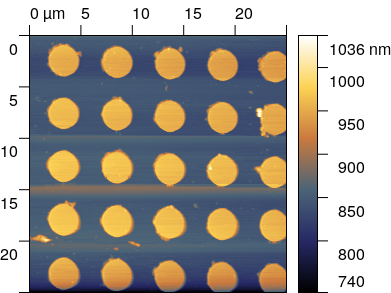
\includegraphics[width=\textwidth]{tm_points}
\caption{Points surface}
\label{fig:}
\end{subfigure}
\begin{subfigure}[b]{0.45\textwidth}
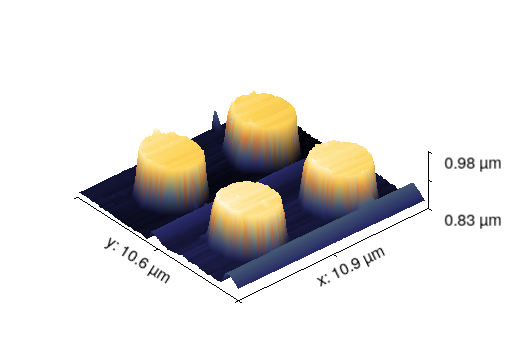
\includegraphics[width=\textwidth]{tm_points_3D}
\caption{Points surface, 3D plot}
\label{fig:sm_raws}
\end{subfigure}\\\vspace{.2cm}
\begin{subfigure}[b]{0.45\textwidth}
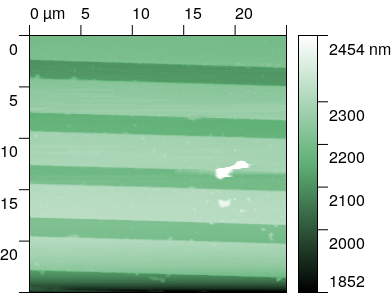
\includegraphics[width=\textwidth]{tm_raws}
\caption{Raws surface}
\label{fig:}
\end{subfigure}
\begin{subfigure}[b]{0.45\textwidth}
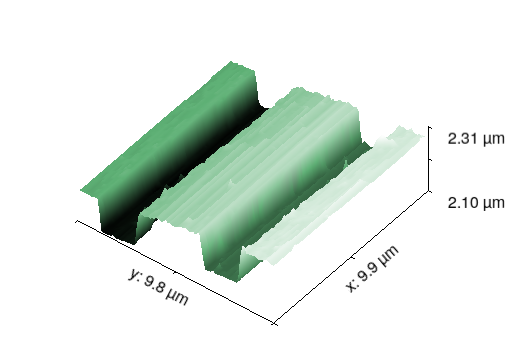
\includegraphics[width=\textwidth]{tm_raws_3D}
\caption{Raws surface, 3D plot}
\label{fig:}
\end{subfigure}\\\vspace{.2cm}
\begin{subfigure}[b]{0.45\textwidth}
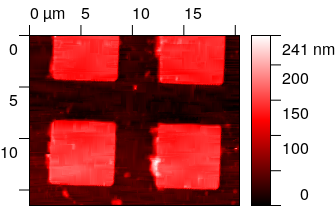
\includegraphics[width=\textwidth]{tm_squares}
\caption{Squares surface}
\label{fig:}
\end{subfigure}
\begin{subfigure}[b]{0.45\textwidth}
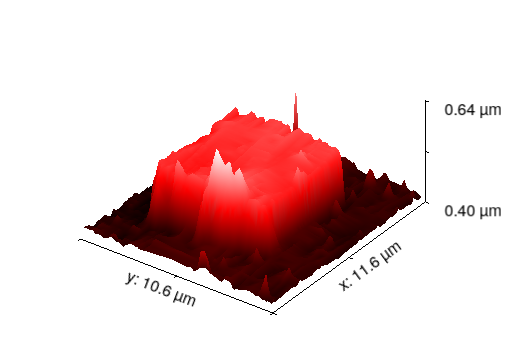
\includegraphics[width=\textwidth]{tm_squares_3D}
\caption{Squares surface, 3D plot}
\label{fig:sm_border}
\end{subfigure}
\caption{Some pictures of the calibration sample}\label{fig:: tm cal}
\end{figure}
As we can see, the data obtained is in agreement with the ones picked up with static mode. The height of the plots are in both modes around $16\mu m$. The corners are a bit less rounded in this mode, we can notice this fact comparing Figure~\ref{fig:3d_and_read_value} with the 3-dimensional plot in Figure~\ref{fig:: tm cal}.

\subsubsection{Sample 1}
In the following picture we can see the picture resulting from the data got about the first sample.
\begin{figure}[H]
\centering
\begin{subfigure}[b]{0.45\textwidth}
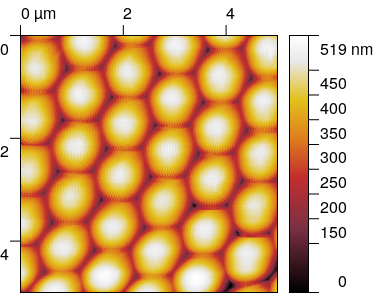
\includegraphics[width=\textwidth]{tm_sample1}
\caption{Sample 1 in tapping mode}
\label{fig:}
\end{subfigure}
\begin{subfigure}[b]{0.45\textwidth}
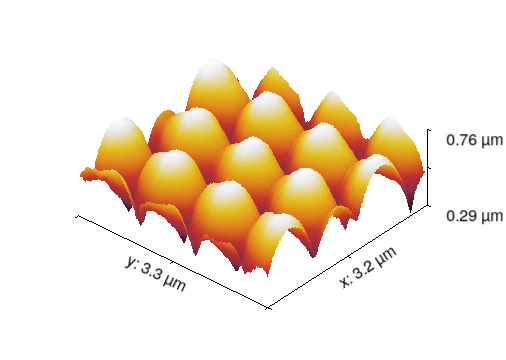
\includegraphics[width=\textwidth]{tm_sample1_3D}
\caption{Sample 1 in tapping mode, 3D plot}
\label{fig:}
\end{subfigure}
\end{figure}

In this case the height is not perfectly in agreement with the one obtained by means of the static mode. With the tapping mode we can measure $43\mu m$ while with the static mode we have $56\mu m$. Anyway the plot that we can observe is in accordance in both the modes.
\subsubsection{Sample 2}
Here we have the data from the second sample.
\begin{figure}[H]
\centering
\begin{subfigure}[b]{0.45\textwidth}
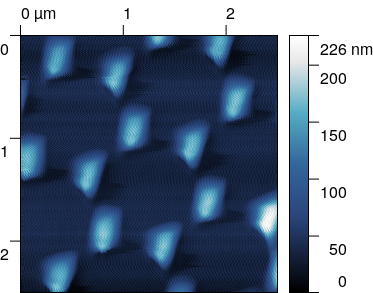
\includegraphics[width=\textwidth]{tm_sample2}
\caption{Sample 2 in tapping mode}
\label{fig:}
\end{subfigure}
\begin{subfigure}[b]{0.45\textwidth}
\includegraphics[width=\textwidth]{tm_sample2_3D}
\caption{Sample 2 in tapping mode, 3D plot}
\label{fig:}
\end{subfigure}
\end{figure}

The plot reminds even in this case a set of stars. The difference of height of the corners of the stars is in this case of only $2\mu m$ ($19\mu m$ in the static mode and $17\mu m$ in the tapping one); we can conclude the agreement between the 2 sets of data.

\subsubsection{Sample 3}
Finally we can see the pictures obtained from the third sample.
\begin{figure}[H]
\centering
\begin{subfigure}[b]{0.45\textwidth}
\includegraphics[width=\textwidth]{tm_sample3}
\caption{Sample 3 in tapping mode}
\label{fig:}
\end{subfigure}
\begin{subfigure}[b]{0.45\textwidth}
\includegraphics[width=\textwidth]{tm_sample3_3D}
\caption{Sample 3 in tapping mode, 3D plot}
\label{fig:}
\end{subfigure}
\end{figure}

In this case we can state that the plot of the material is not very regular. In fact, we probably measured 2 differents part of the sample with the 2 modes. The resulting data have a difference of the maximum height really relevant: $9.4nm$ in static mode versus $44nm$ in tapping mode.

At this point we attach a table of the heights measured thanks to Gwyddion (as far as the 3 samples are concerned we will write the maximum height).

\begin{figure}[ht]
\begin{center}
\includegraphics[scale=0.4]{table.png}
\end{center}
\end{figure}

Comparing the table with the pictures, we can see that it is not always clear from the images to extimate the height. Actually, even the data reported here are not very precise because of the peaks and hills; it is not always clear from which 2 points to measure the z-distance because the surfaces are often not regular.

In conclusion, we show the distance between the centers of the cells measured from the data got in both the modes. As we can see, the values are in good agreement between them.
\begin{table}[ht]
\begin{center}
    \caption{Distances between centers}
    \label{tab:table2}
    \begin{tabular}{l|c|r} % <-- Alignments: 1st column left, 2nd middle and 3rd right, with vertical lines in between
      \textbf{Mode} & \textbf{Sample 1} & \textbf{Sample 2}\\
       & distances in $\mu m$ & distances in $\mu m$ \\
      \hline
      Static & 1.018 & 1.126\\
      Tapping & 1.040 & 1.0598\\
      
    \end{tabular}
  \end{center}
\end{table}
\section{Conclusions}
We have studied and understand the working principle of AFM, as well as the two most common operation modes: static or contact mode, and tapping or dynamic mode. We have read about and recognize the most common artifacts in AFM images. Finally, we have used the compact NaioAFM both in static and tapping mode to measure three different samples, after optimizing the PID values using a calibration sample. Better results were obtained in the tapping mode, probably due to the fact that we had some issues with the contact mode tip. The Naiosurf software provided with the AFM was used to captured the raw data, and the open source software Gwyddion was utilized to process the images (filtering, background correction, coloring...) and obtain the final ones presented in the report.

\nocite{*}
\vfill
\bibliographystyle{unsrt}
\bibliography{references}
\end{document}